\documentclass[main]{subfiles}

\begin{document}

\chapter{Aplicación web}

La interfaz en forma de página web podría considerarse la forma secundaria de acceder a Faborez, debido a que aunque pueden realizarse casi todas las operaciones del cliente Android carece de funcionalidades como las notificaciones. Además, la necesidad de configurar el navegador, o de dar una dirección de forma manual, dificultan la obtención de la localización del usuario. De esta forma, se pierde gran parte del valor que tiene el servicio.

\section{Interfaz del usuario}

A continuación se describen las distintas partes que tiene esta aplicación web, enumerando las partes de la interfaz web y detallando la funcionalidad que cada una ofrece. Se acompaña a cada una una captura de pantalla como ejemplo.

\paragraph{Pantalla de \emph{login}}
La interfaz que se muestra inicialmente al acceder a la web de Faborez. Su única funcionalidad es comenzar el proceso de autenticación mediante Google+, tal y como se indica en el \cref{sec:arquitectura-autenticación} (ver \cref{fig:webapp-login}).

\begin{figure}
  \centering
  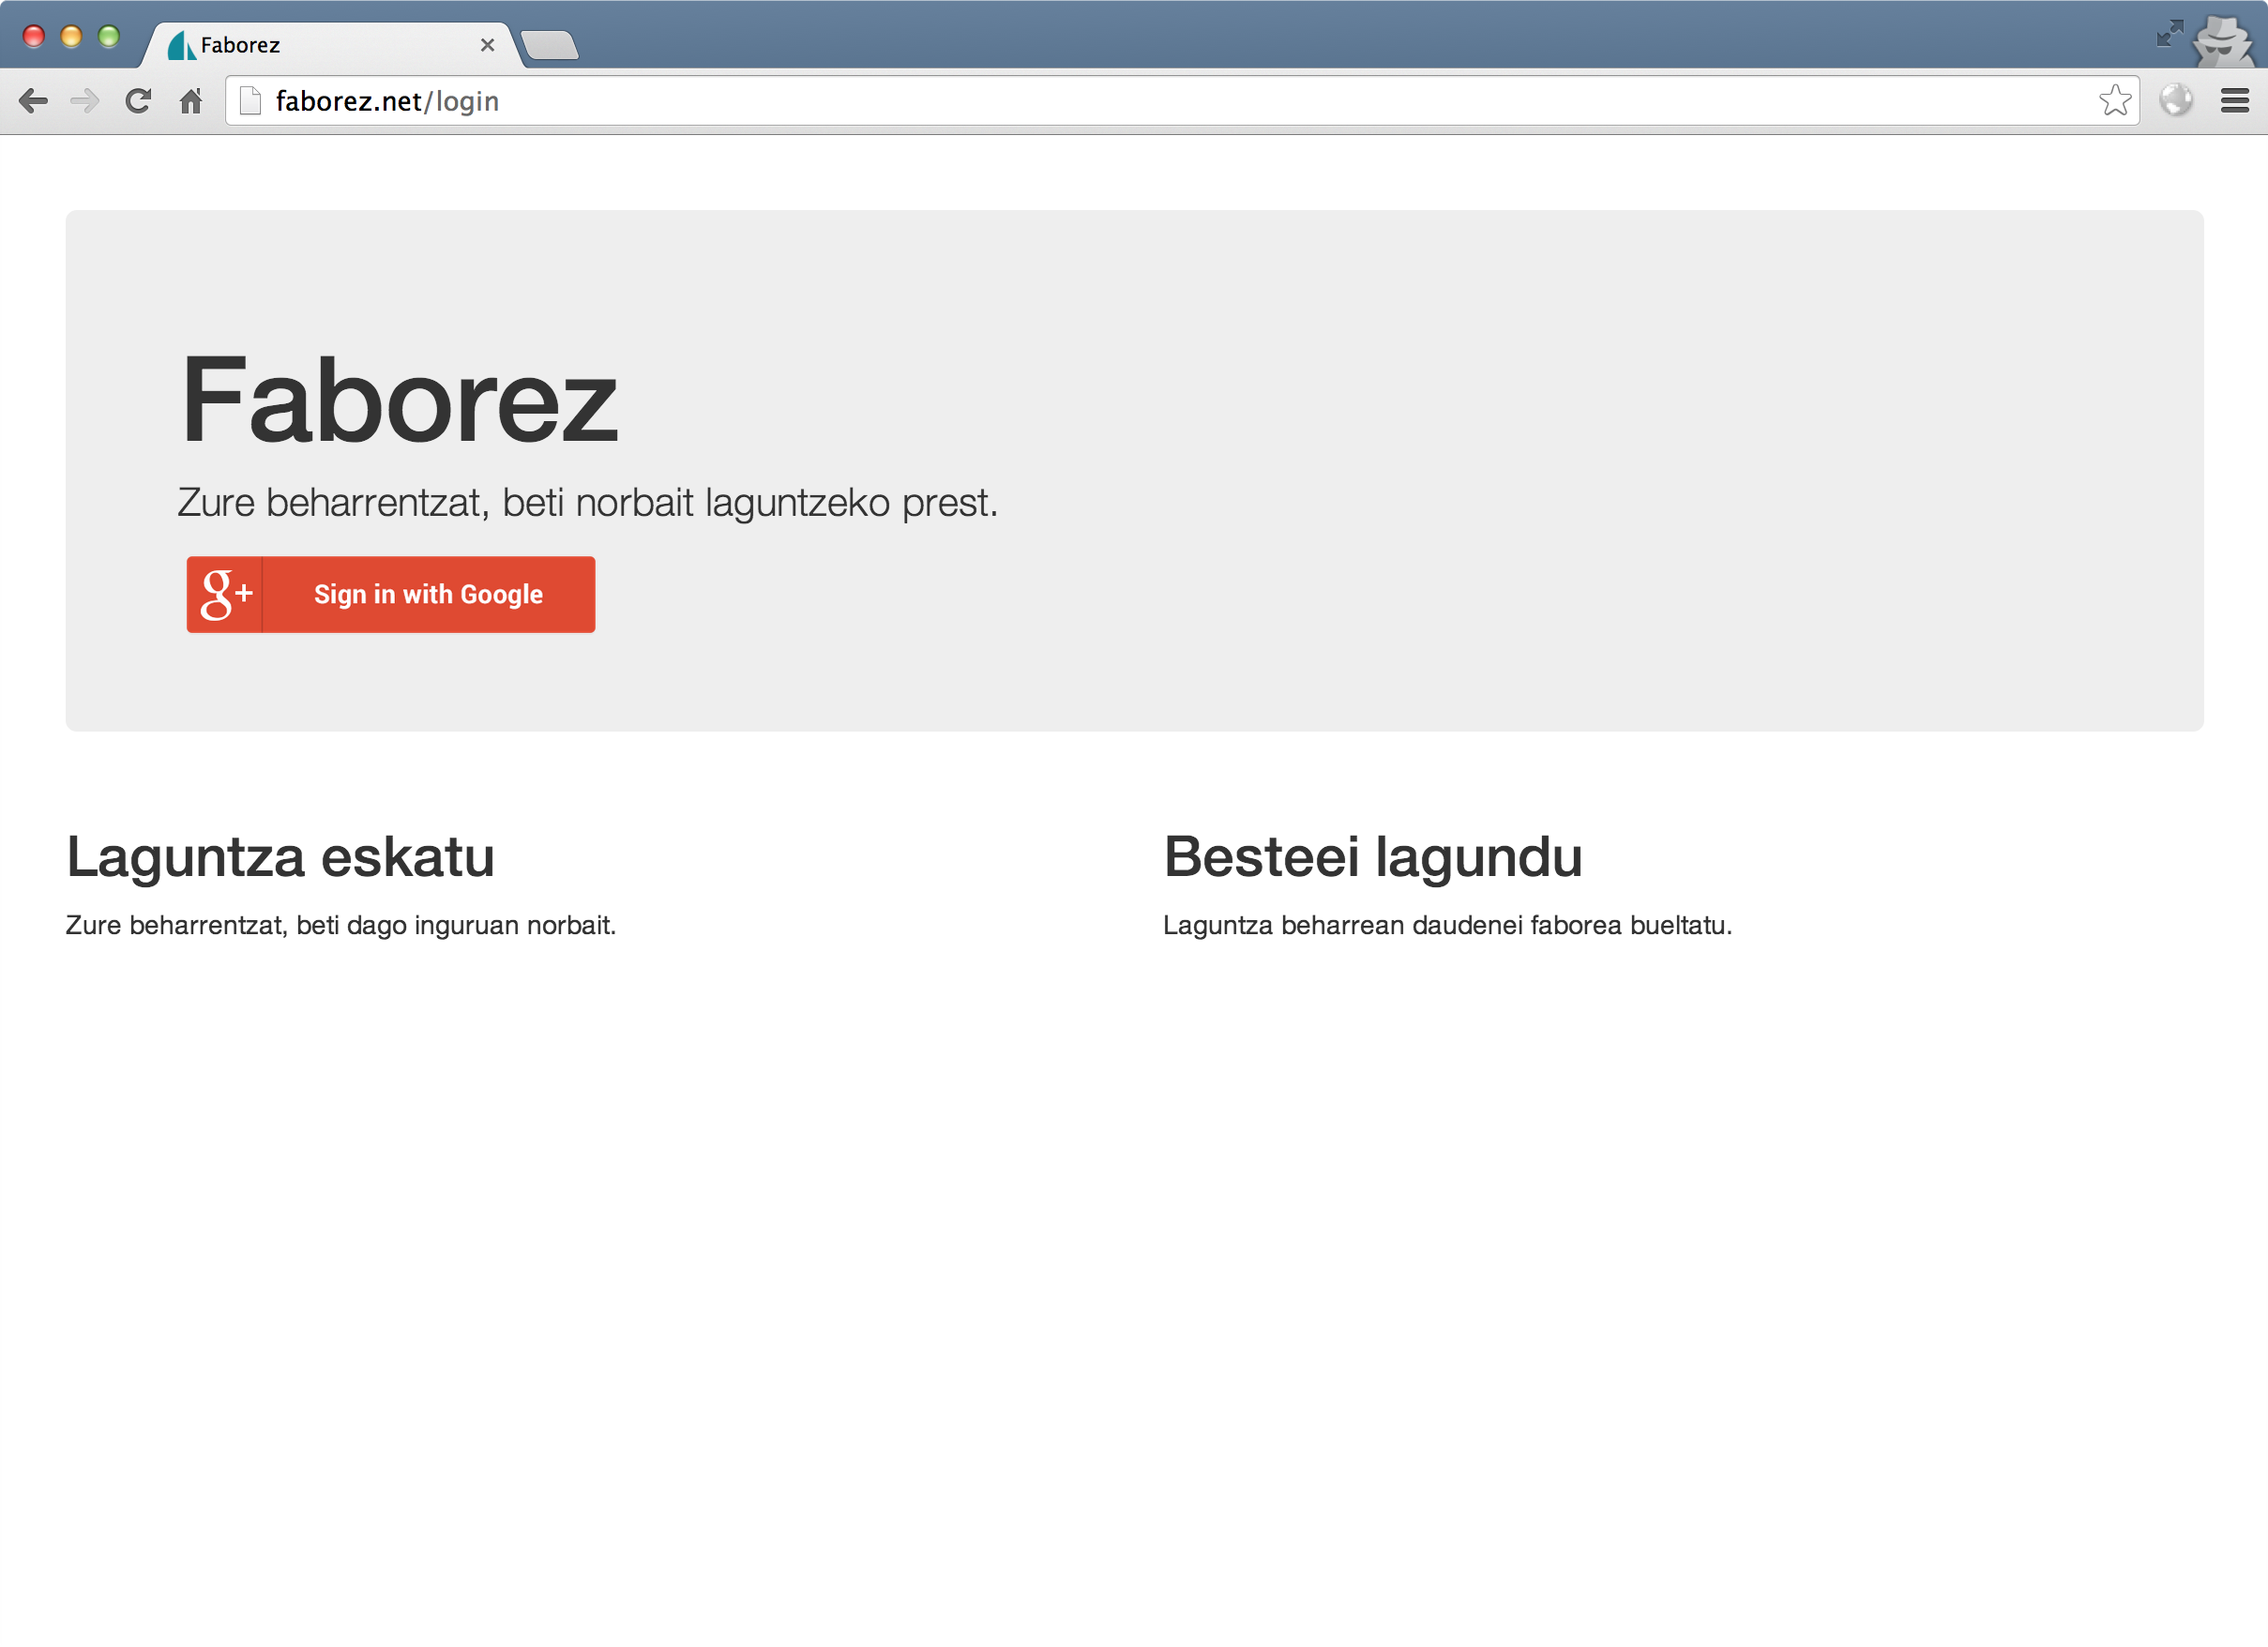
\includegraphics[width=0.9\textwidth]{images/webapp-login}
  \caption{Interfaz de \emph{login}}
  \label{fig:webapp-login}
\end{figure}

\paragraph{Pantalla principal}
En ella se muestran, una vez obtenida la localización del usuario, las peticiones de favor más cercanas con los datos más relevantes y el enlace para acceder a las mismas. En otra pestaña, se encuentra el formulario para añadir nuevas peticiones (ver \cref{fig:webapp-newform}).

\begin{figure}
  \centering
  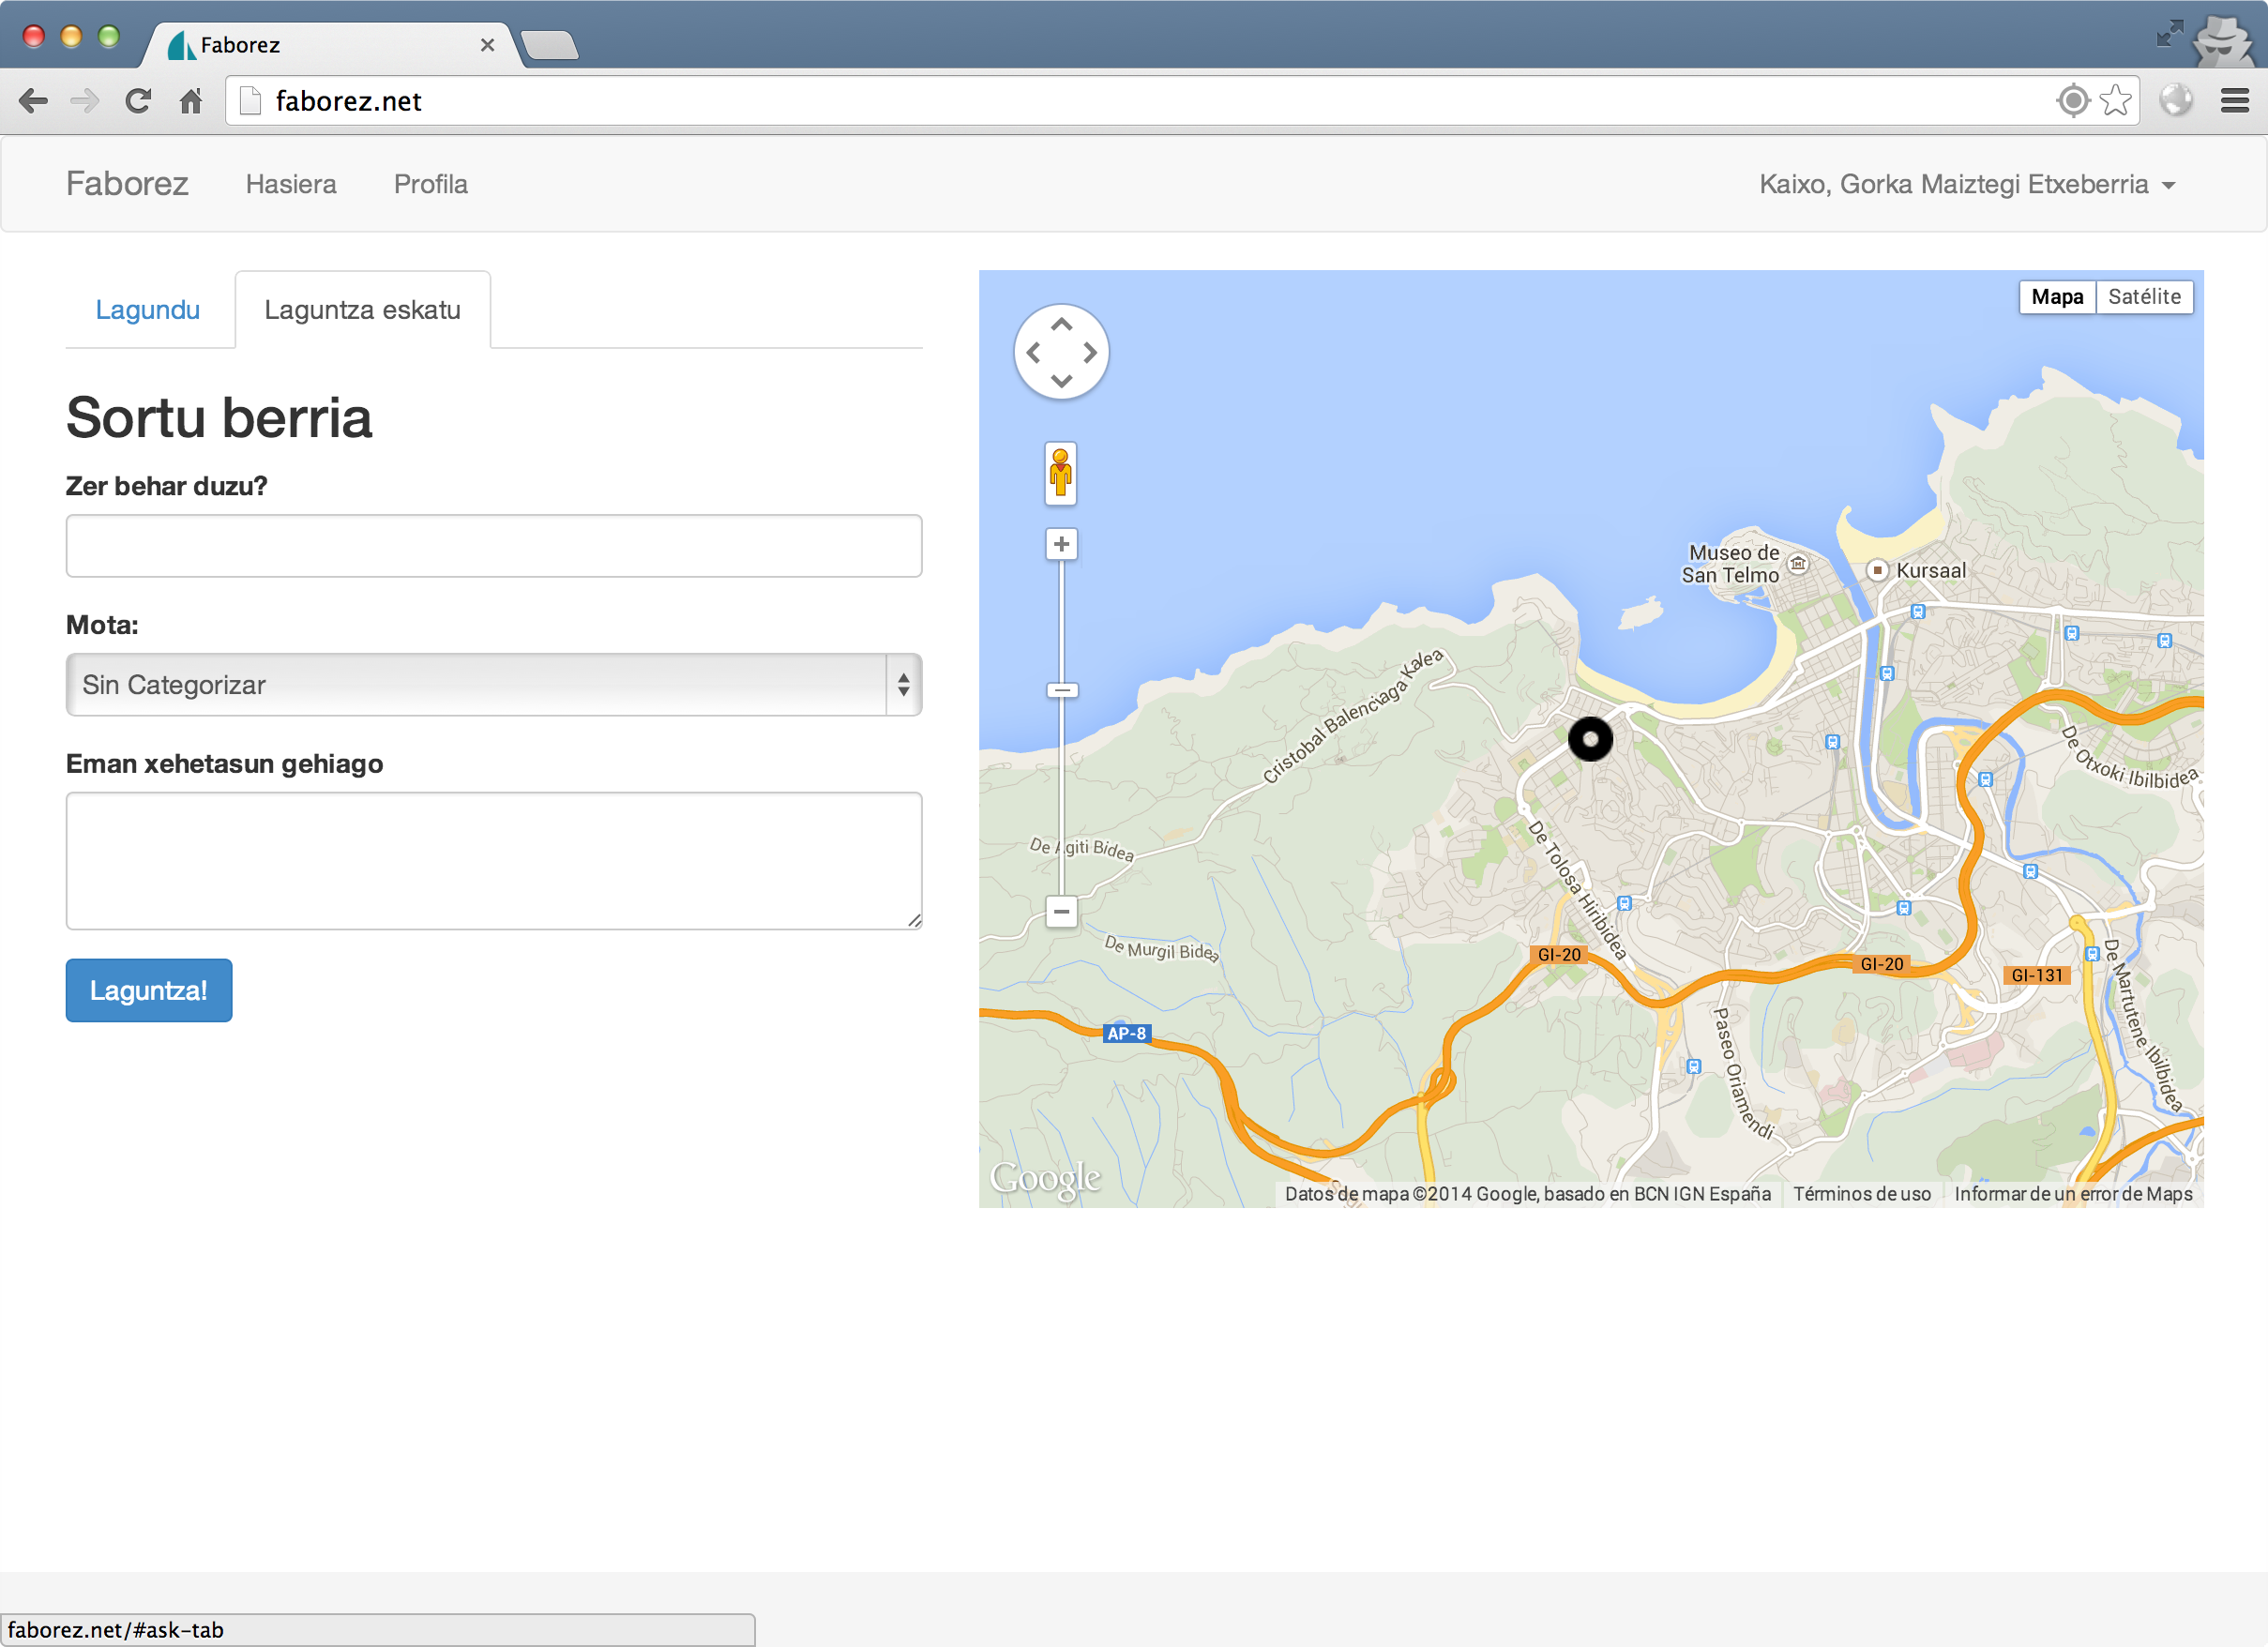
\includegraphics[width=0.9\textwidth]{images/webapp-newform}
  \caption{Pantalla principal}
  \label{fig:webapp-newform}
\end{figure}

\paragraph{Visualización de petición}
Esta pantalla muestra todos los detalles sobre una petición en concreto. Si la petición es del propio usuario, se muestran todas las respuestas, junto con el botón de entrar a la conversación (ver \cref{fig:webapp-request}).

\begin{figure}
  \centering
  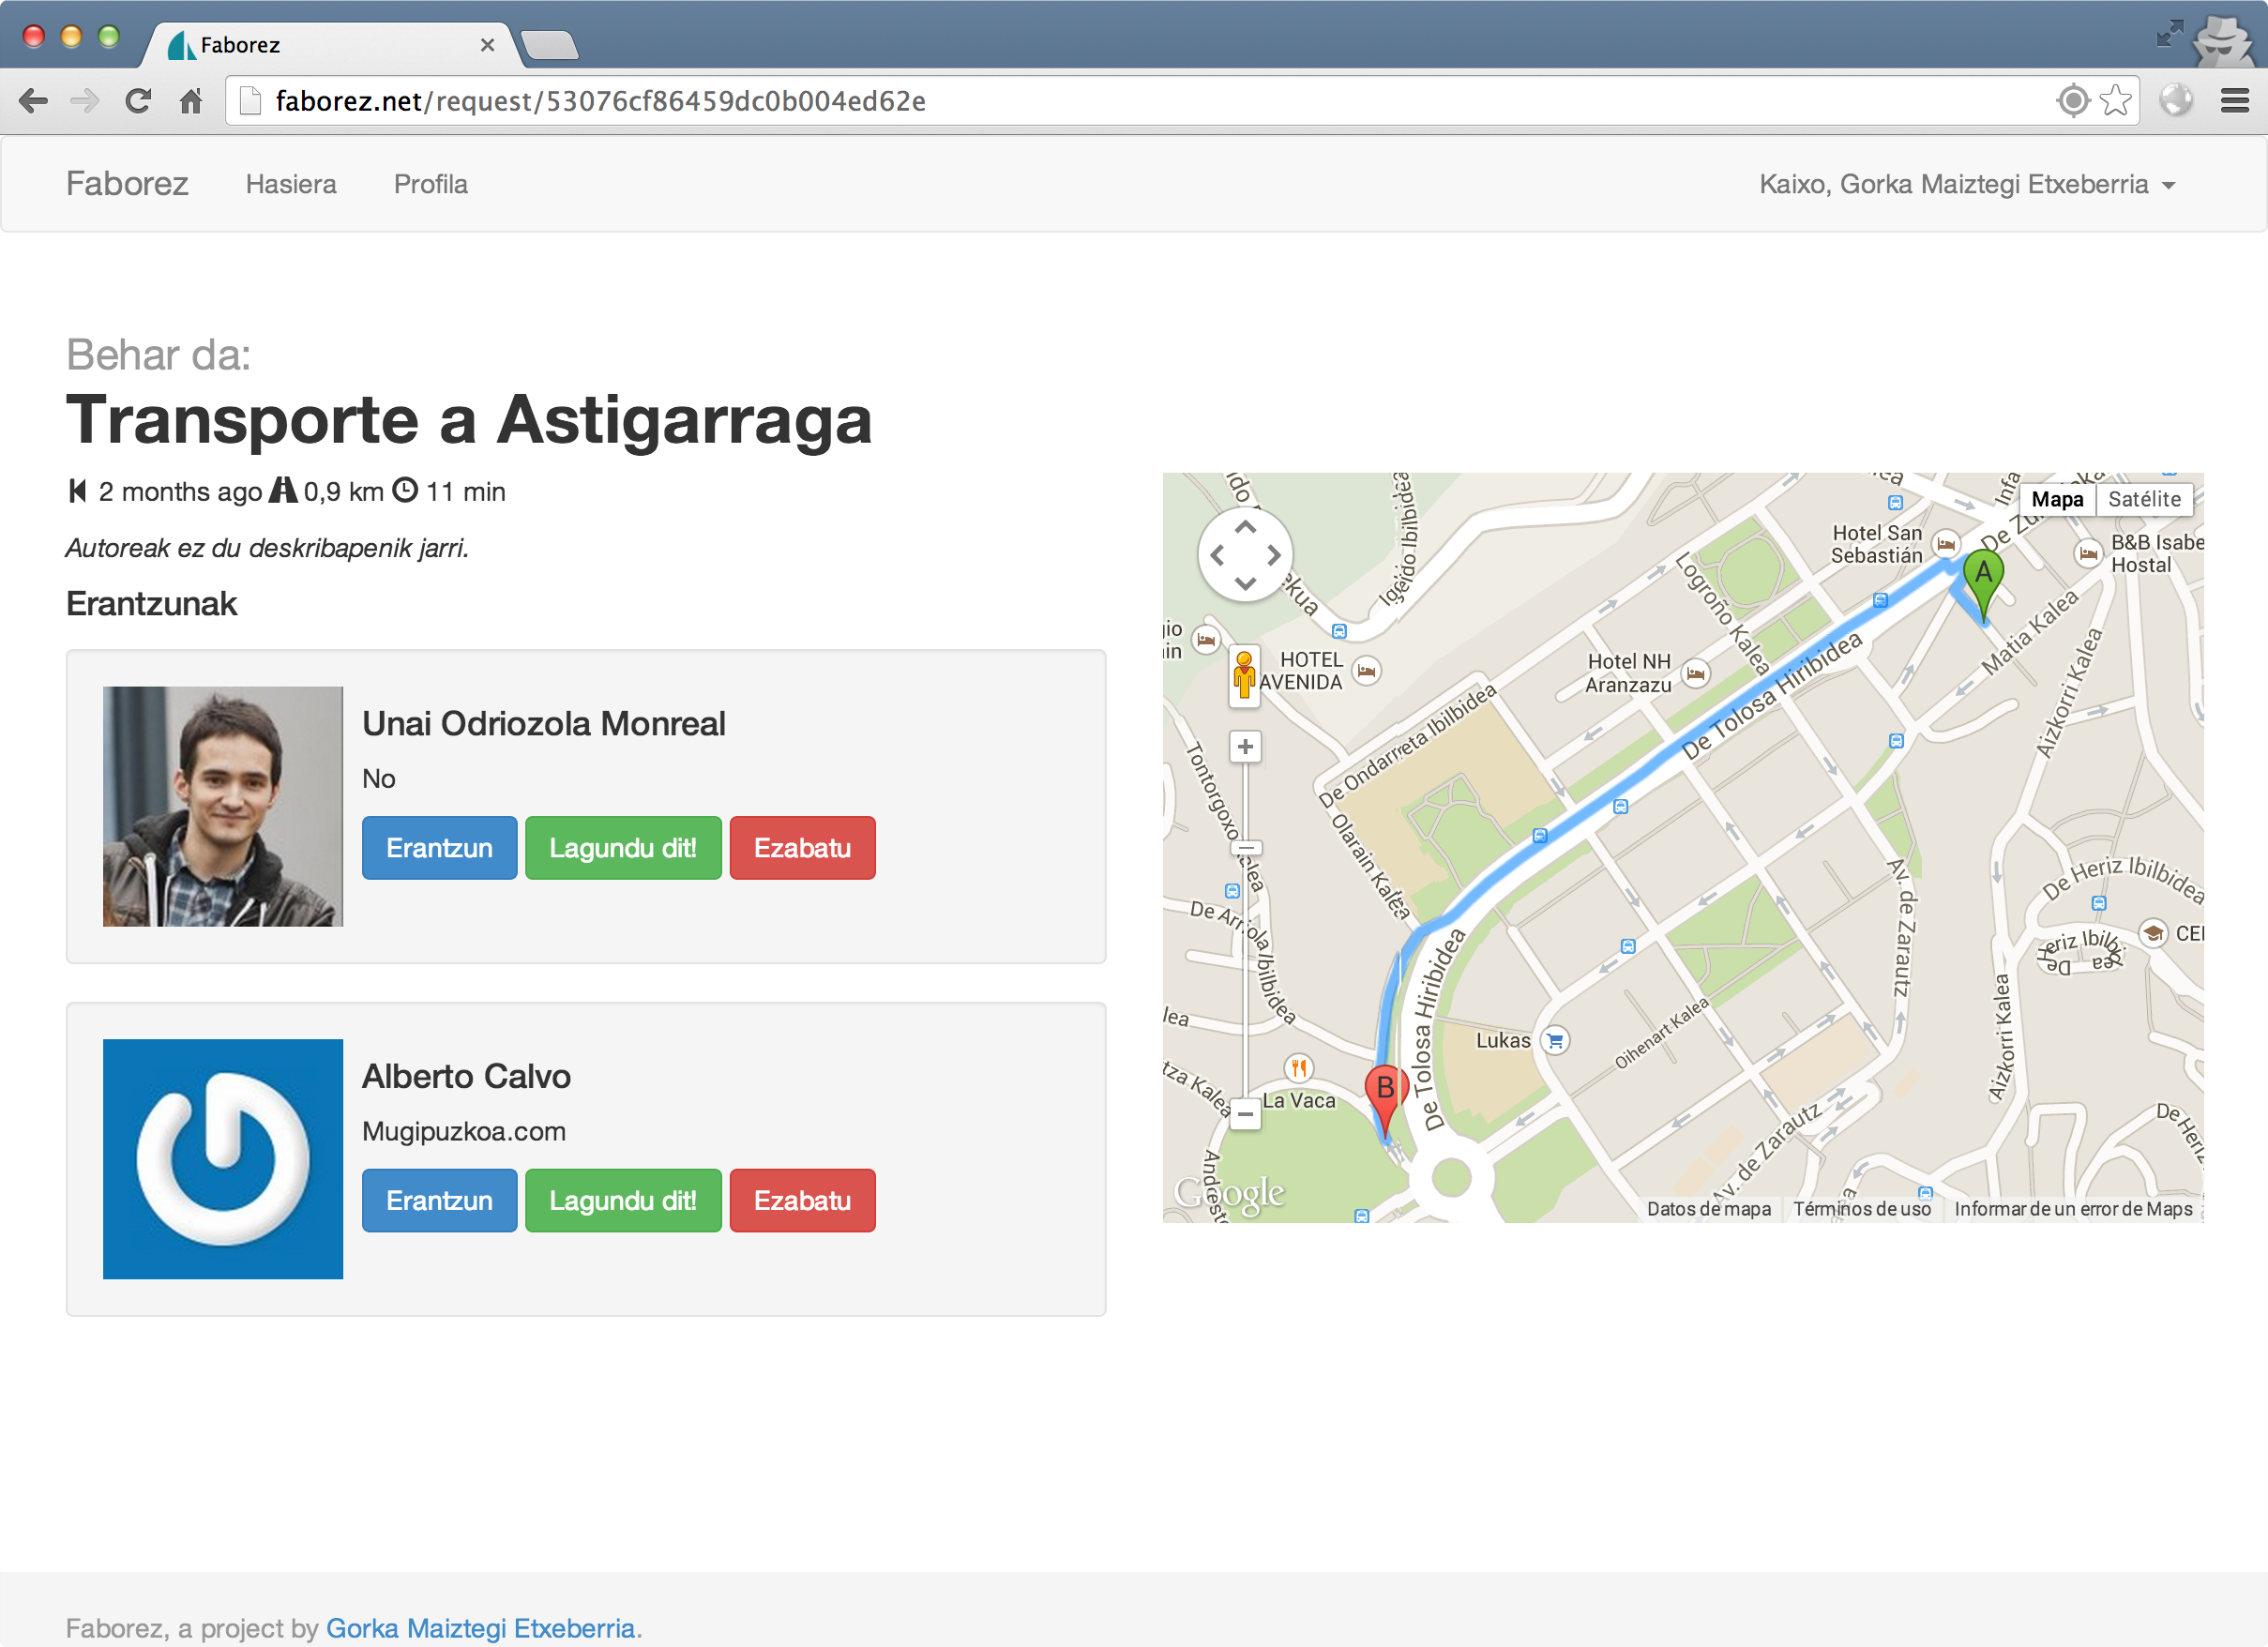
\includegraphics[width=0.9\textwidth]{images/webapp-request}
  \caption{Visualización de la petición}
  \label{fig:webapp-request}
\end{figure}

\paragraph{Hilo de mensajes}
Al igual que en la aplicación Android, se muestran los mensajes intercambiados entre el usuario y la persona que respondió a la petición. Desde esta interfaz es posible responder con más mensajes o navegar a su perfil de usuario (ver \cref{fig:webapp-reply}).

\begin{figure}
  \centering
  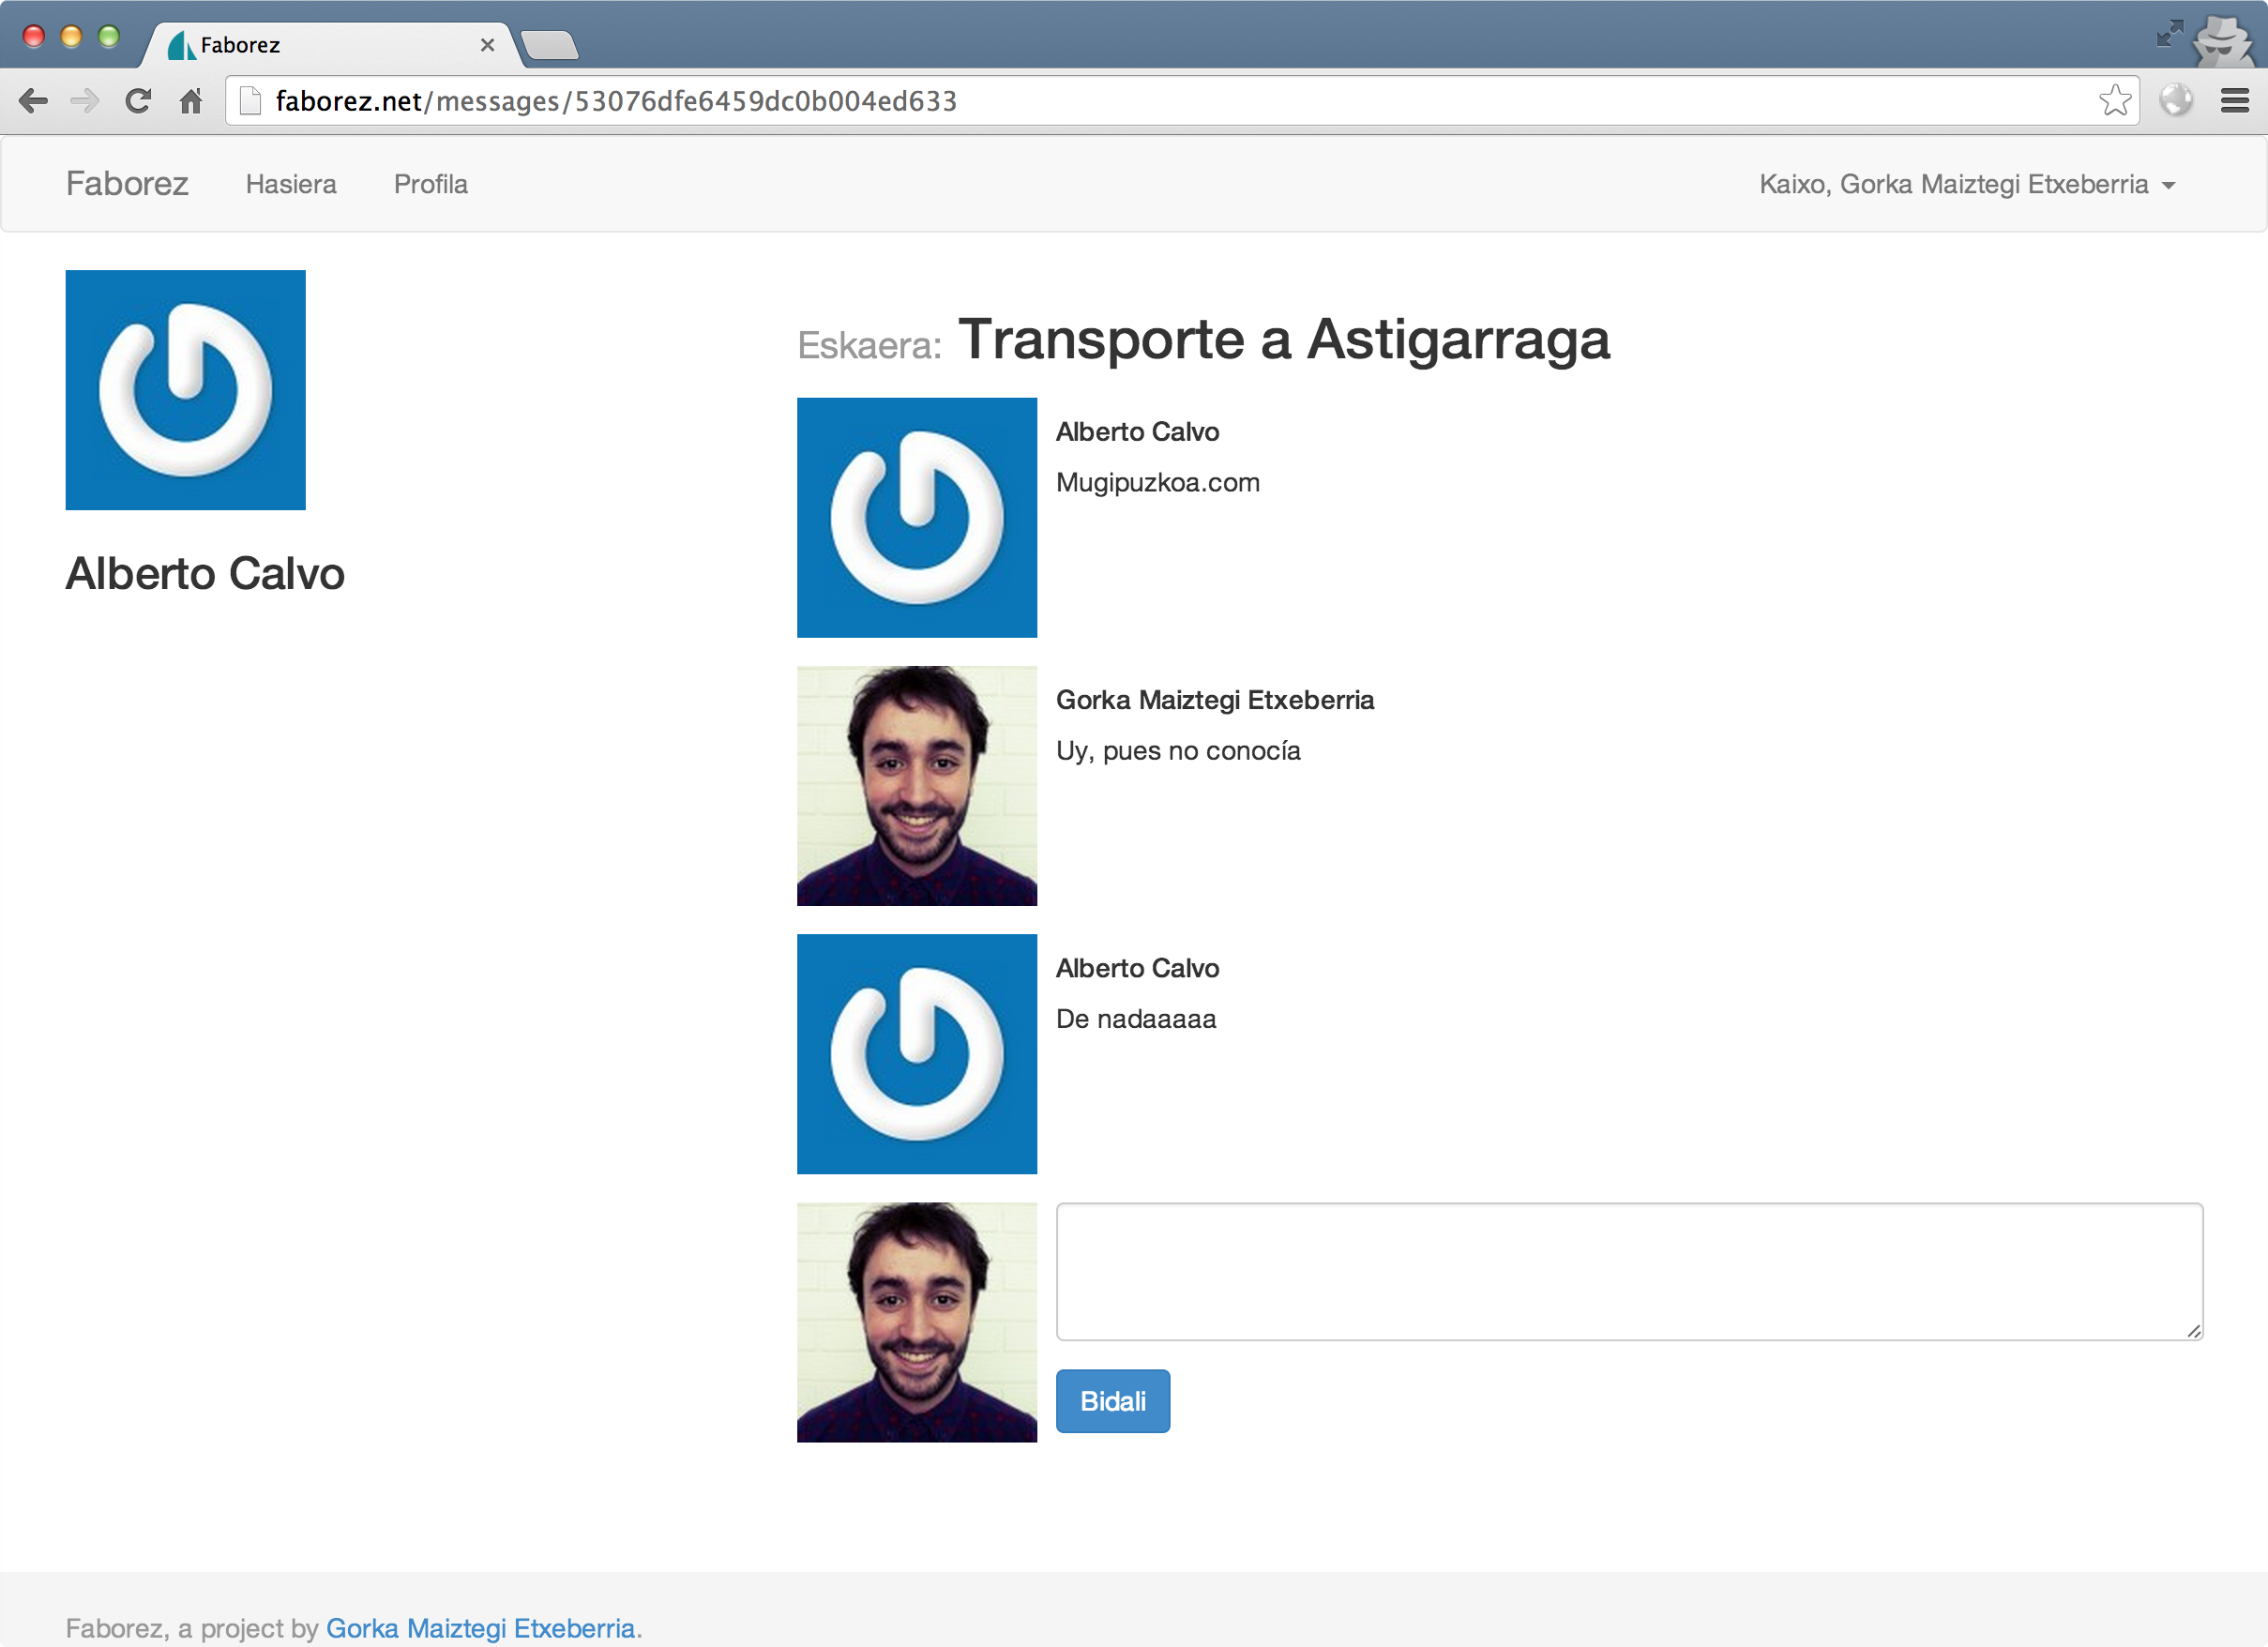
\includegraphics[width=0.9\textwidth]{images/webapp-reply}
  \caption{Hilo de respuestas}
  \label{fig:webapp-reply}
\end{figure}

\paragraph{Perfil de usuario}
En el perfil del usuario se puede visualizar información básica acerca de éste, junto con la actividad que ha tenido en Faborez, mostrando las peticiones de favor que ha realizado (ver \cref{fig:webapp-user}).

\begin{figure}
  \centering
  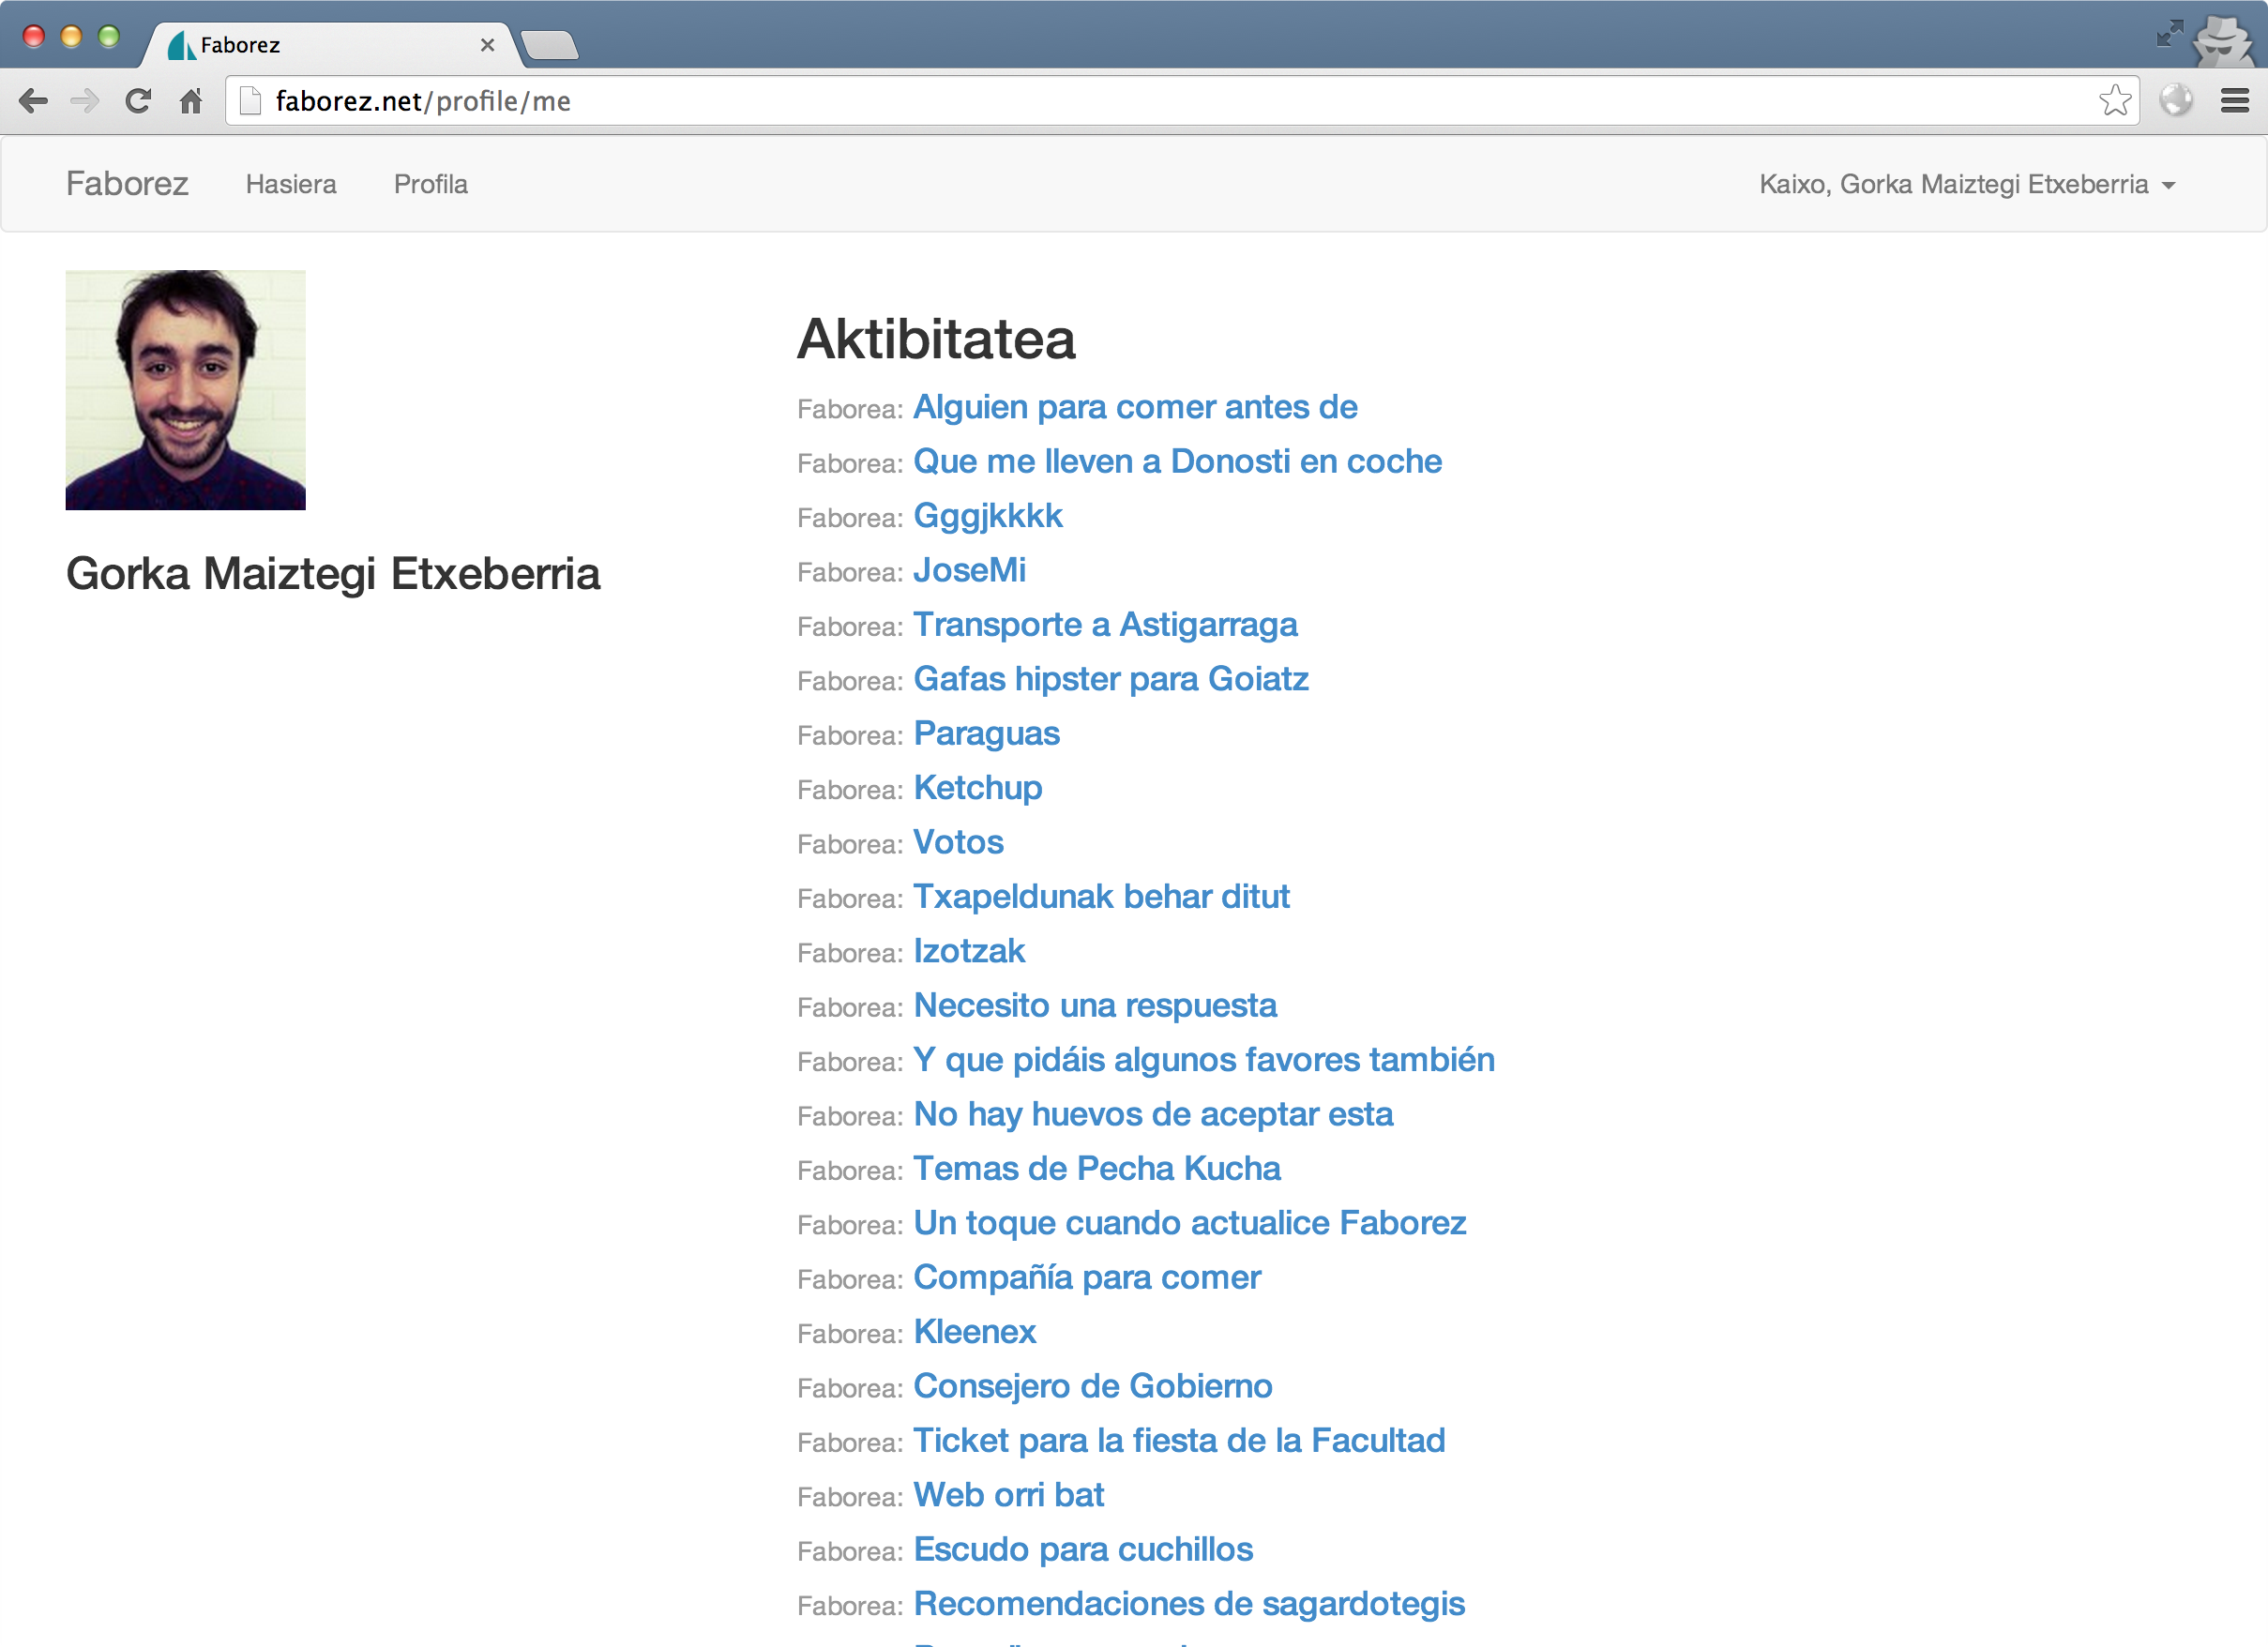
\includegraphics[width=0.9\textwidth]{images/webapp-user}
  \caption{Perfil del usuario}
  \label{fig:webapp-user}
\end{figure}

\section[Utilización de APIs]{Utilización de \glspl{api}}

La aplicación hace uso de dos librerías para completar el funcionamiento de algunas de las interfaces. Estas son la \gls{api} de geolocalización~\autocite{geolocation-api} y el \enquote{API de rutas de Google}~\autocite{google-directions-api}, utilizadas en dos partes distintas de la aplicación.

En el primer caso, la \gls{api} de geolocalización es la forma estándar de \gls{html5} para obtener la localización. El usuario deberá dar permiso explícitamente al navegador, mostrándole una alerta para ello. Con la información obtenida, se envían las coordenadas al servidor para descargar las peticiones de favor más cercanas.

La utilidad de Google es utilizada en la interfaz de detalle de la petición, valiéndose de la localización del usuario, muestra en el mapa de la parte derecha la ruta más corta a pie hasta la posición de la petición de favor, además de mostrar los datos relativos a la ruta, distancia y tiempo, en la información que se muestra.

\end{document}
